\chapter{Introduction to Graphs}

Some data is easiest to work with if we imagine it as a set of \newterm{nodes} connected by \newterm{edges}.  For example,  on some social networks each user can follow any number of other users.  We can think of each user as node and the edge points from the user who follows to the user they follow:

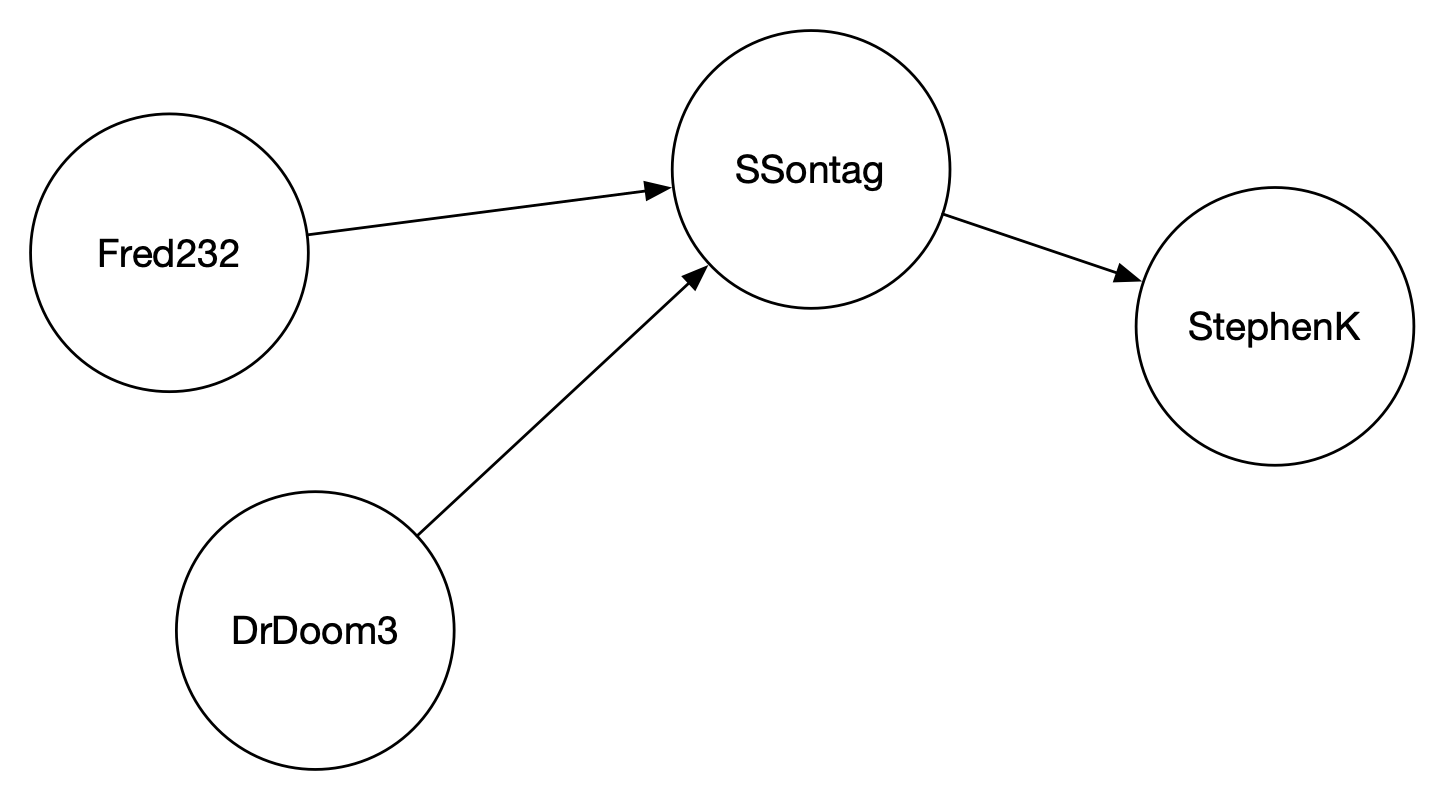
\includegraphics[width=0.7\textwidth]{simpledirected.png}

This diagram shows four users and three follows.   Following  is a directed relationship: Fred232 follows SSontag, but SSontag doesn't follow Fred232.   So we would way that this is a \newterm{directed graph} with four nodes and three edges.

There are also undirected graphs.  for example,  you can imagine a graph that represents big data lines between cities.  All the big data lines allow communications in both directions:

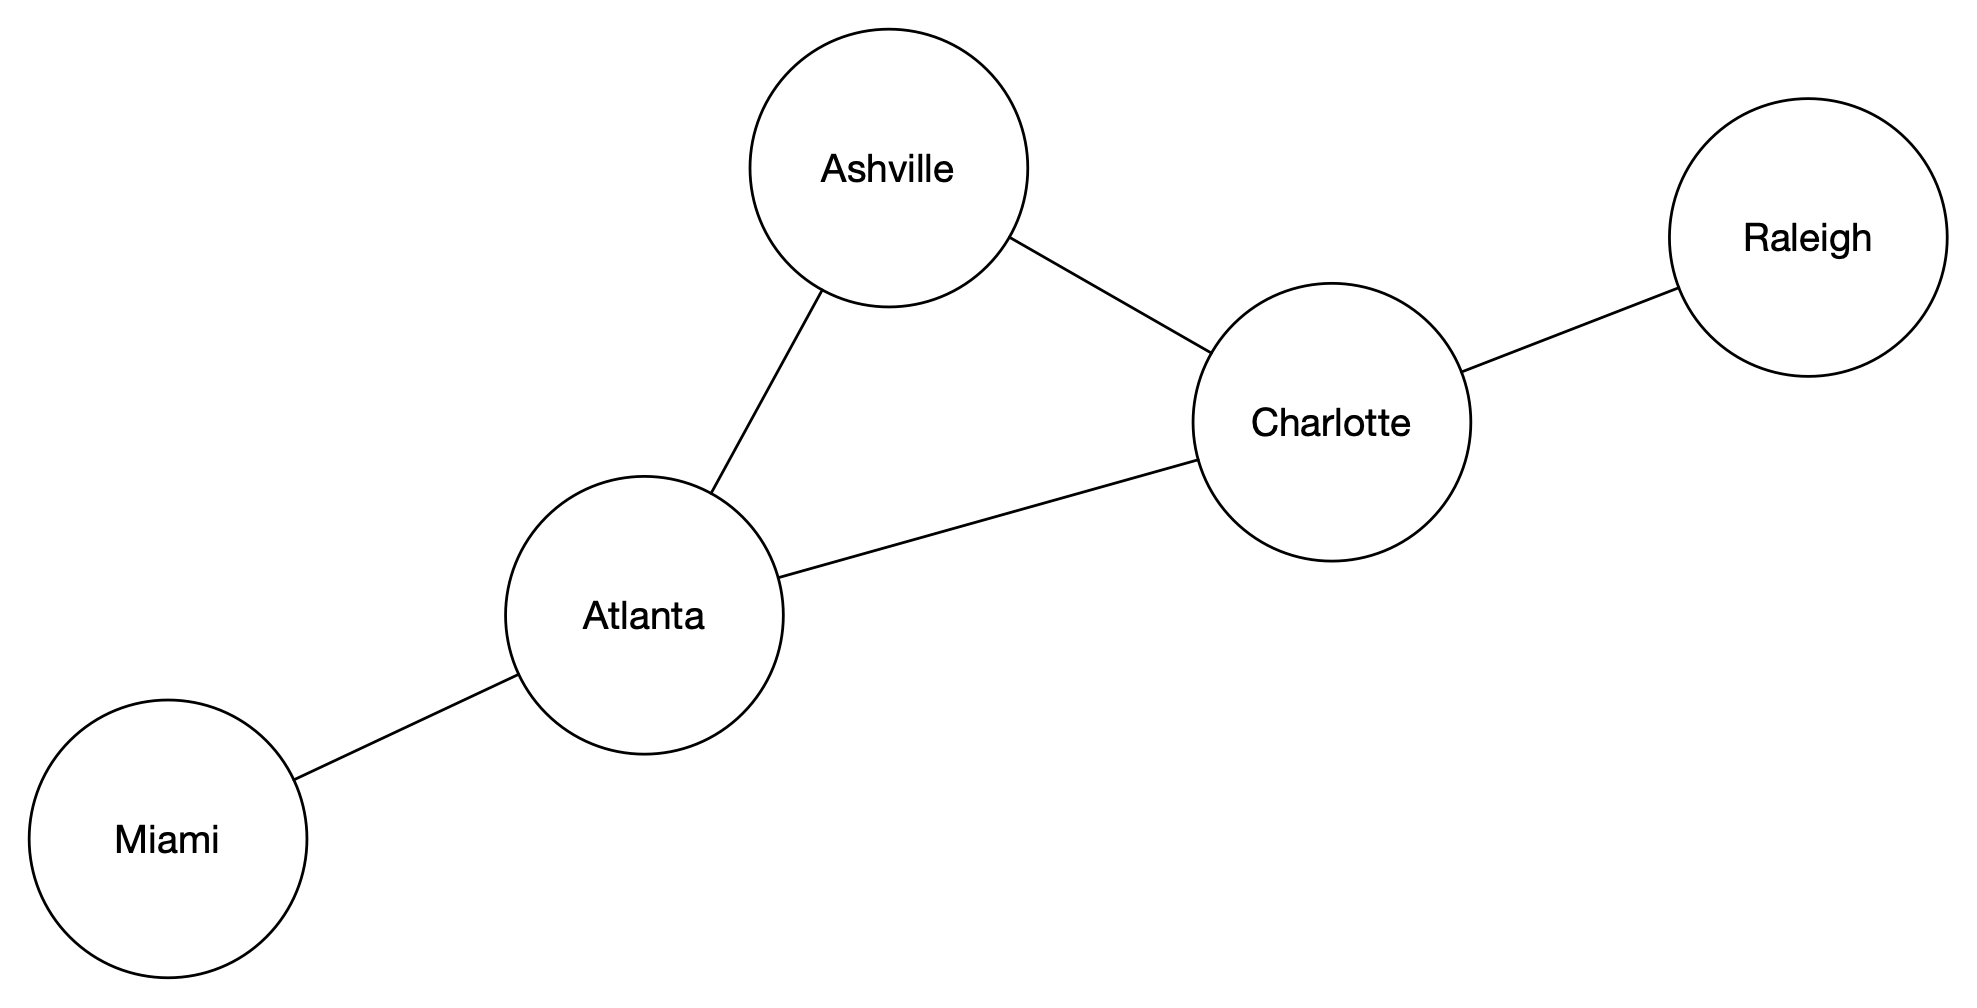
\includegraphics[width=0.7\textwidth]{simpleundirected.png}

The arrows are gone: if data can flow from Charlotte to Raleigh, then data can flow from Raleigh to Charlotte.

There is a whole branch of mathematics called \newterm{Graph Theory} that studies the properties of graphs.  Here are two questions that we might ask about this graph:
\begin{itemize}
\item What is the shortest number of edges that we would need to follow to get from Miami to Raleigh?
\item Does the graph have any paths where you could end up where you started? This is called a \newterm{cycle}.  This graph has one cycle: Atlanta $\rightarrow$ Asheville $\rightarrow$ Charlotte $\rightarrow$ Atlanta.
\end{itemize}

There are even database systems that are specifically designed to hold and analyze graph data.  Not surprisingly,  these are called \newterm{Graph Databases}.

Some graphs are \newterm{connected}: you can get from one node to any other node by following edges.  Is this graph connected?

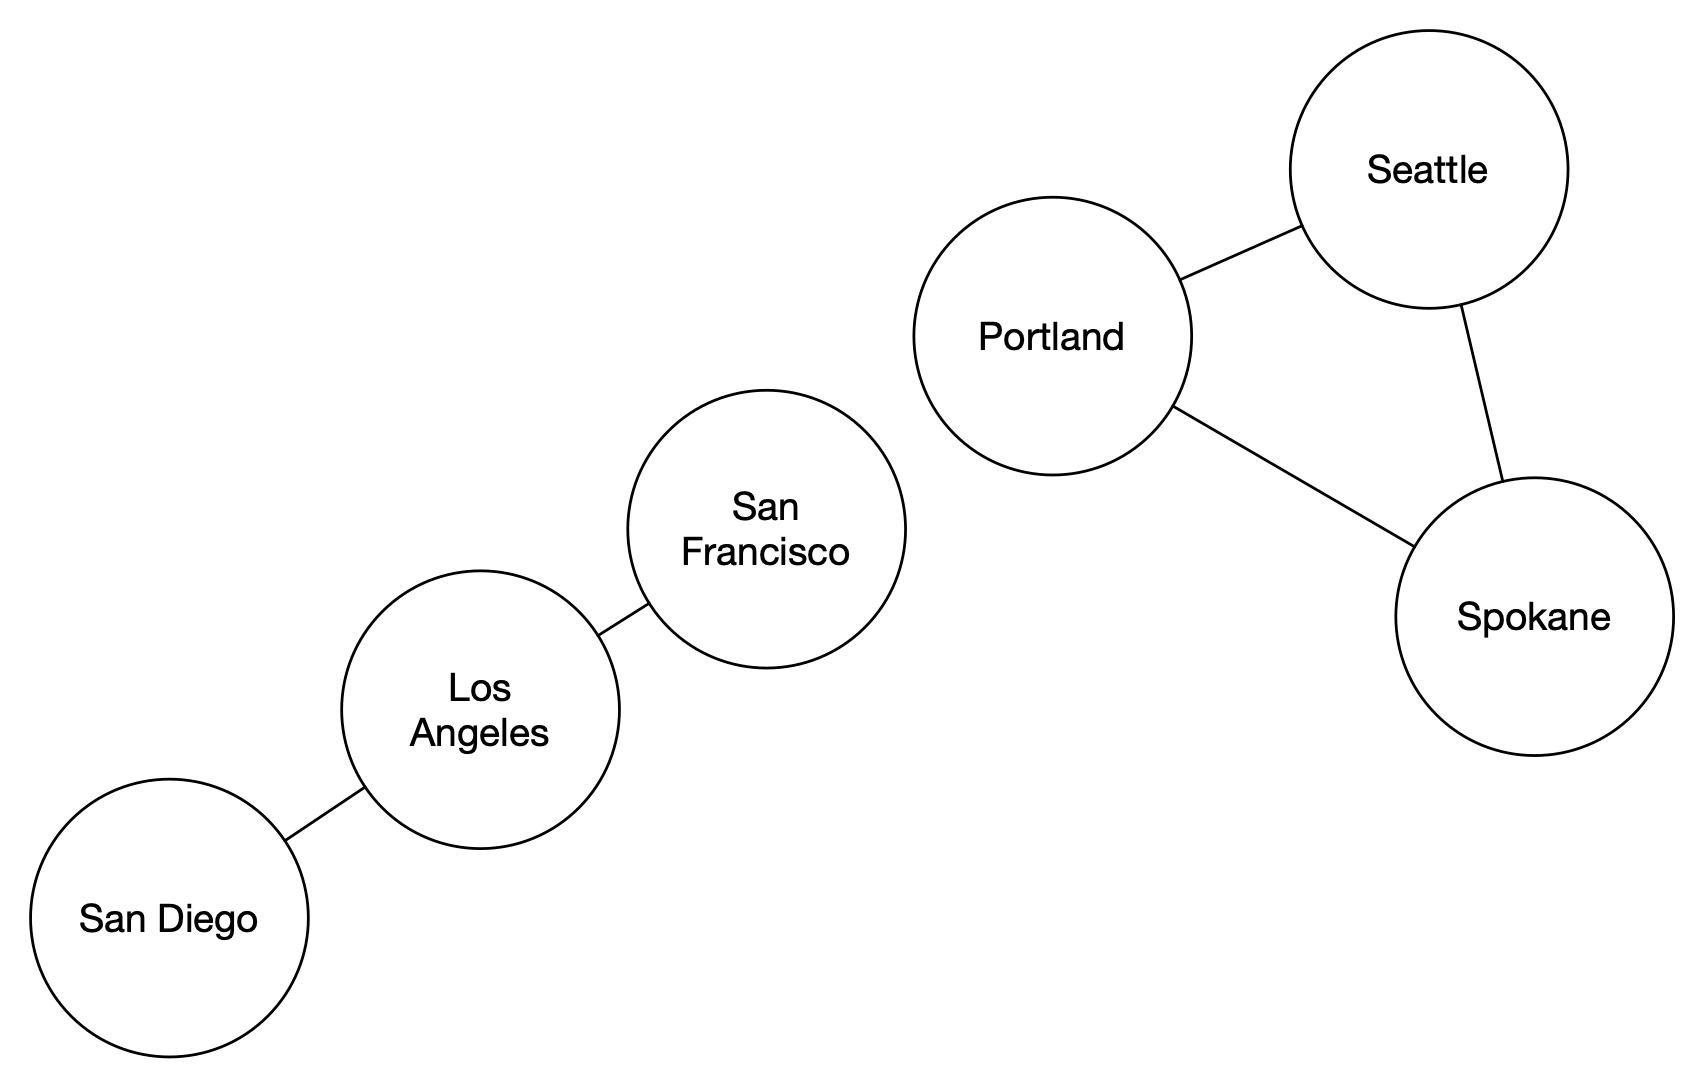
\includegraphics[width=0.7\textwidth]{notconnected.png}

This graph is \textit{not} connected! You can't follow edges from San Diego to Seattle.

In graph data,   the nodes and edges often have attributes.  For example,  a node representing a city might have a name and a population.  An edge representing a data line might have a bandwidth (bits per second) and a latency (how many nanoseconds between when you put a bit into the pipe and when it comes out the other end.).

\section{Finding Good Paths}

For a lot of problems, we are trying to find the best path from one node to another.  If all the edges are the same,  this usually means finding the path that requires walking the fewest edges.

Sometimes the edges have a cost attribute.  For example,  you might want to find the cheapest way to ship a container from New York City to Long Beach, Calif.   In this case the nodes are train depots.  Each train line between the depots has a cost.  What is the cheapest path?

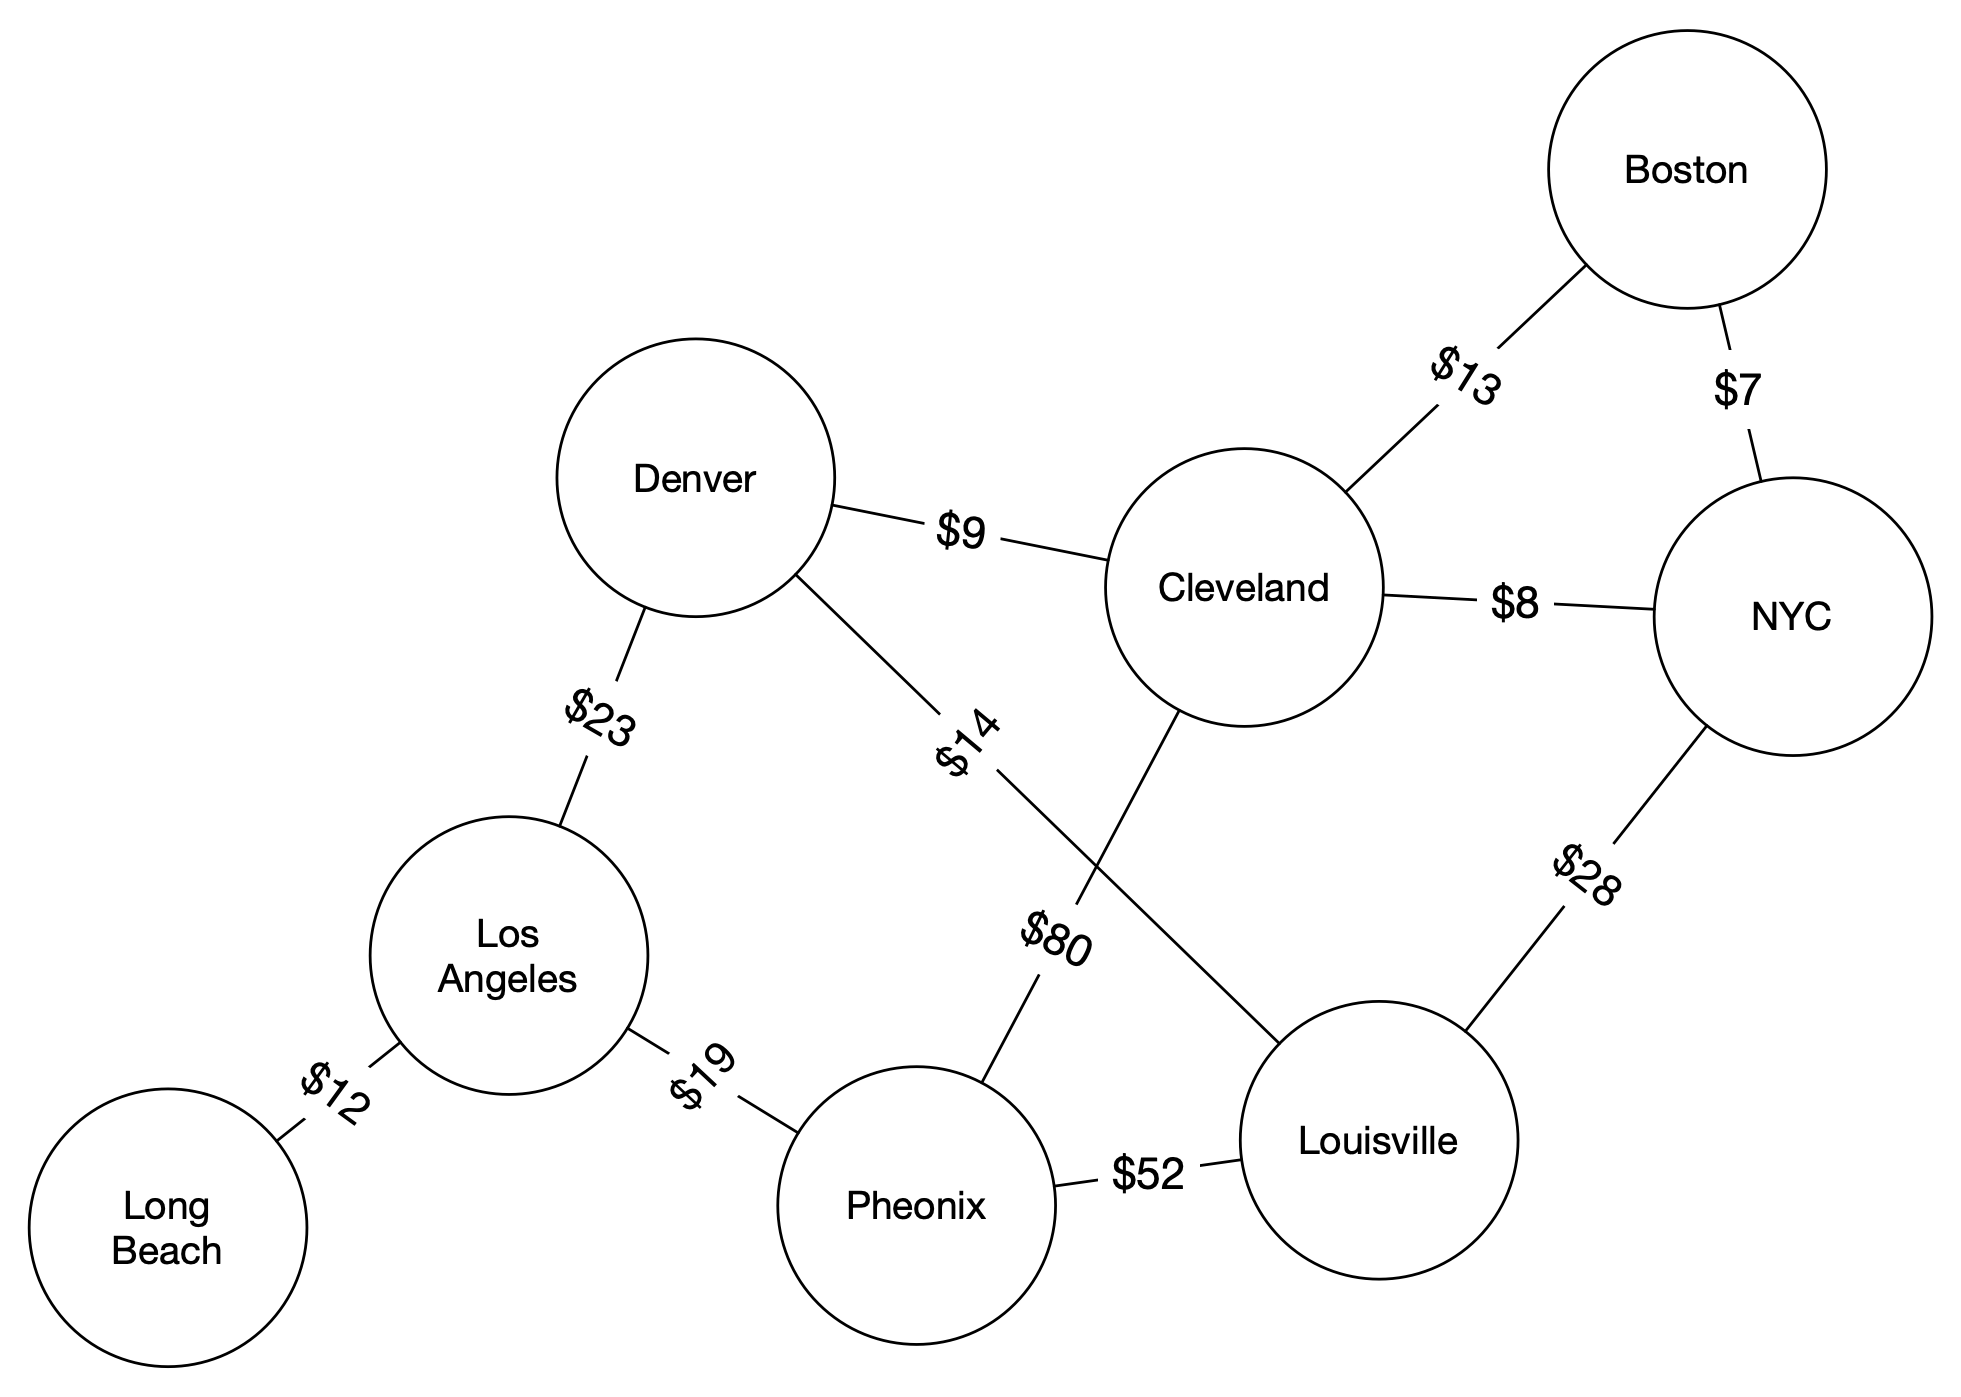
\includegraphics[width=0.7\textwidth]{depots.png}

(You don't need to solve this; that's what we have computers for!)

The graphs that you see here are really small, so finding efficient paths isn't difficult. -- you could just try all of them! However, in many computer programs,  we are working with millions of nodes and edges.  Efficient graph algorithms are \textit{really} important.  You will implement one of them in the next chapter.



